\documentclass[a4paper,12pt]{article} % добавить leqno в [] для нумерации слева
\usepackage[a4paper,top=1.3cm,bottom=2cm,left=1.5cm,right=1.5cm,marginparwidth=0.75cm]{geometry}
%%% Работа с русским языком
\usepackage{cmap}					% поиск в PDF
\usepackage{mathtext} 				% русские буквы в фомулах
\usepackage[T2A]{fontenc}			% кодировка
\usepackage[utf8]{inputenc}			% кодировка исходного текста
\usepackage[english,russian]{babel}	% локализация и переносы

\usepackage{graphicx}

\usepackage{wrapfig}
\usepackage{tabularx}

\usepackage{hyperref}
\usepackage[rgb]{xcolor}
\hypersetup{
colorlinks=true,urlcolor=blue
}
\usepackage{multirow}
\usepackage{hhline}


%%% Дополнительная работа с математикой
\usepackage{amsmath,amsfonts,amssymb,amsthm,mathtools} % AMS
\usepackage{icomma} % "Умная" запятая: $0,2$ --- число, $0, 2$ --- перечисление

%% Номера формул
\mathtoolsset{showonlyrefs=true} % Показывать номера только у тех формул, на которые есть \eqref{} в тексте.

%% Шрифты
\usepackage{euscript}	 % Шрифт Евклид
\usepackage{mathrsfs} % Красивый матшрифт

%% Свои команды
\DeclareMathOperator{\sgn}{\mathop{sgn}}

%% Перенос знаков в формулах (по Львовскому)
\newcommand*{\hm}[1]{#1\nobreak\discretionary{}
{\hbox{$\mathsurround=0pt #1$}}{}}

\begin{document}

\newenvironment{lines}[1][\textwidth] % по умолчанию линейки на всю ширину текста
{
\newcolumntype{E}{>{}p{#1}<{\hrulefill}} % в конце нашего столбца будет приписываться \hrulefill
\begin{flushright} % автоматически вставим flushright
\begin{tabular}[h]{E} % и tabular нужного формата
}
{\end{tabular}\end{flushright}
}
	
	\begin{titlepage}
	\begin{center}
		{\large МОСКОВСКИЙ ФИЗИКО-ТЕХНИЧЕСКИЙ ИНСТИТУТ (НАЦИОНАЛЬНЫЙ ИССЛЕДОВАТЕЛЬСКИЙ УНИВЕРСИТЕТ)}
	\end{center}
	\begin{center}
		{\large Физтех-школа электроники, фотоники и молекулярной физики}
	\end{center}
	
	
	\vspace{4.5cm}
	{\huge
		\begin{center}
			{Лабораторная работа 5.5.1}\\
			 {Измерение коэффициента ослабления потока $ \gamma $-лучей в веществе и определение их энергии}
		\end{center}
	}
	\vspace{2cm}
	\begin{flushright}
		{\LARGE Салтыкова Дарья \\
			\vspace{0.5cm}
			Б04-105}
	\end{flushright}
	
	\vspace{0.5cm}
	
	\begin{lines}[.5
	\textwidth]
  {\LARGE Допуск} \rule{6.5cm}{0.25pt} \vspace{0.5cm}\\
 {\LARGE Выполнение} \rule{3cm}{0.25pt}\vspace{0.5cm} \\ {\LARGE Сдача} \rule{3cm}{0.25pt} \\ % \rule сделает линейку указанной длины и толщины
\end{lines}
	\vspace{6cm}
	\begin{center}
		Долгопрудный 2023
	\end{center}
\end{titlepage}

\section{Цель работы}
С помощью сцинтилляционного счетчика измерить линейные коэффициенты ослабления потока $ \gamma $-лучей в свинце, железе и алюминии; по их величине определить энергию $ \gamma $-квантов.
	
\section{Теоретические сведения}
\noindent Гамма-лучи возникают при переходе возбужденных ядер из одного энергетического состояния в другое, более низкое. Энергия $ \gamma $-квантов обычно заключена между несколькими десятками килоэлектронвольт и несколькими миллионами электрон-вольт. Гамма-кванты не несут электрического заряда, их масса равна нулю. Проходя через вещество, пучок $ \gamma $-квантов постепенно ослабляется. Ослабление происходит по экспоненциальному закону, который может быть записан в двух эквивалентных нормах:
	
	\begin{equation}\label{I(mu)}
	I = I_0 e^{-\mu l}, \quad I_o e^{-\mu 'm_1} 
	\end{equation}
	
	\medskip
	
\noindent В этих формулах $ I, I_0 $ --- интенсивности прошедшего и падающего излучений, $ l $ --- длина пути, пройденного пучком гамма-лучей, $ m_1 $ ---
	масса пройденного вещества, приходящаяся на единицу площади, $ \mu $ и
	$ \mu' $ --- константы, величина которых зависит от вещества, сквозь которое проходят гамма-лучи. Длину пути $ l $ обычно выражают в сантиметрах,
	поэтому $ \mu $ имеет размерность см$ ^{-1} $; величину $ m_1 $ измеряют в г/см$ ^2 $,
	так что размерность $ \mu' $ равна см$ ^2 $/г. Форма записи через массу является предпочтительной, потому что $ \mu' $, в отличие от $ \mu $, не зависит от плотности среды. 
	
	\medskip
	
\noindent Ослабление потока гамма-лучей, происходящее при прохождении среды, связано с тремя эффектами: \textbf{фотоэлектрическим поглощением},
	\textbf{комптоновским рассеянием} и с \textbf{генерацией электрон-позитронных пар}. Рассмотрим эти эффекты.
	
	\subsection{Фотоэлектрическое поглощение.} 
	
	\noindent При столкновении гамма-квантов с электронами внутренних атомных оболочек может происходить поглощение квантов. Энергия гамма-кванта передается соответствующему электрону, а импульс делится между этим электроном и оставшимся после
	его вылета ионом. Свободный электрон не может поглотить гамма-квант,
	так как при этом невозможно одновременно удовлетворить законам
	сохранения энергии и импульса. Наружные электроны не принимают участия в фотоэлектрическом поглощении, потому что они слабо
	связаны в атоме, так что их практически можно считать свободными.
	Вероятность $ dP_\text{ф} $ фотоэлектрического поглощения гамма-квантов пропорциональна длине пути $ dl $ и плотности электронов в среде (в расчет
	должны приниматься только электроны, принадлежащие внутренним
	оболочкам атомов):
	
	\begin{equation}\label{mu ph}
	dP_\text{ф} = \sigma_\text{ф} n_1 dl, \quad \mu_\text{ф} = \sigma_\text{ф} n_1
	\end{equation}
	
\noindent Здесь $ n_1 $ --- плотность внутренних электронов, а $ \sigma_\text{ф} $ --- поперечное сечение фотоэлектрического поглощения. Поперечное сечение характеризует вероятность фотоэффекта, рассчитанную на один электрон. Связь между $ \mu_\text{ф} $ и $ \sigma_\text{ф} $ устанавливается из формулы \eqref{I(mu)} и в явном виде определяет зависимости $ \mu $ от плотности среды.

\medskip
	
\noindent Пусть в результате фотоэффекта энергия гамма-кванта передается
	электрону, находящемуся на $ i $-й оболочке атома. Обозначим через $ W_i $
	энергию связи этого электрона. После вылета из атома электрон приобретает кинетическую энергию $ T_i = \hbar \omega - W_i $.
	Освободившееся после вылета электрона место заполняется затем
	одним из электронов с вышележащих оболочек. При таких переходах
	возникает характеристическое рентгеновское излучение.
	
	\begin{wrapfigure}[13]{l}{0.4\linewidth}
		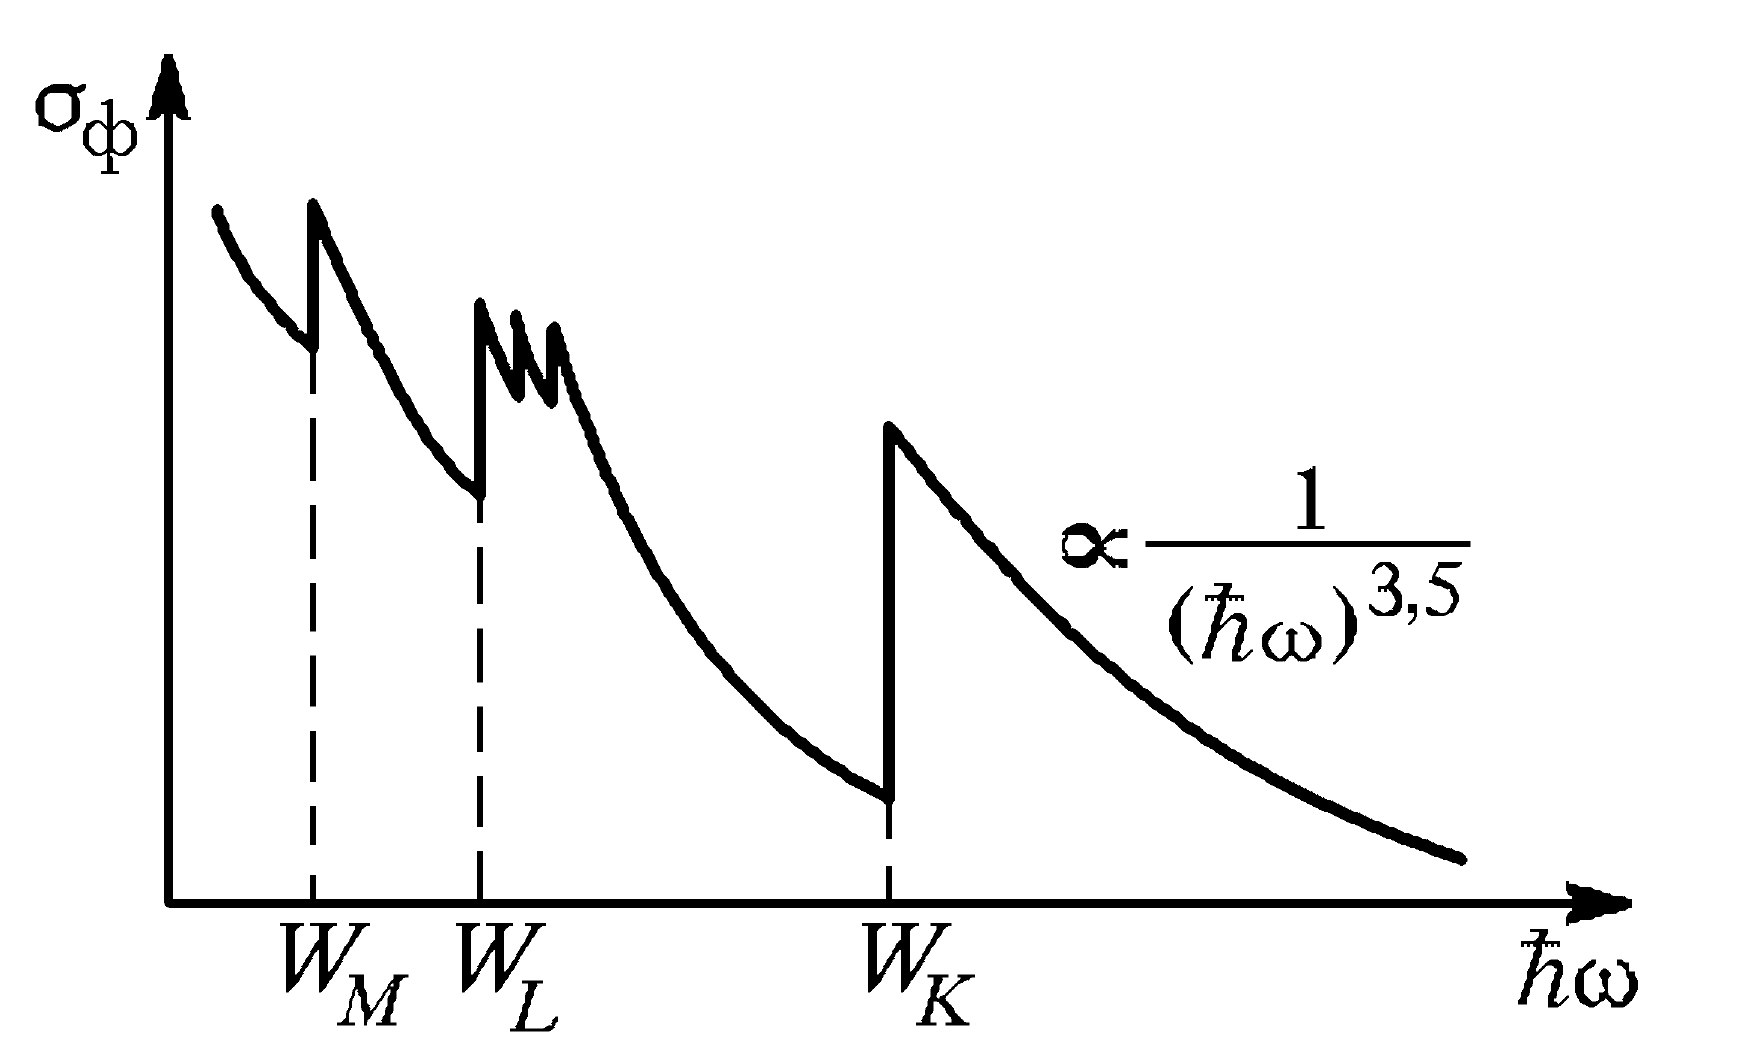
\includegraphics[width=\linewidth]{photo}
		\caption{Зависимость сечения фотоэффекта от энергии гамма-квантов}
		\label{ris photo}
	\end{wrapfigure}
	
	\medskip
	
\noindent Вероятность фотоэффекта сложным образом зависит от энергии
	гамма-лучей и от заряда ядер. Для оценок можно пользоваться формулой
	
	\begin{equation}\label{sigma ph}
	\sigma_\text{ф} \propto \dfrac{Z^5}{(\hbar\omega)^{3,5}}
	\end{equation}
	
\noindent Из формулы \eqref{sigma ph} видно, что вероятность фотоэффекта быстро возрастает при переходе от легких элементов к тяжелым резко падает с увеличением энергии гамма-квантов. На рис. \ref{ris photo} показана энергетическая зависимость сечения фотоэффекта. Из рисунка видно, что при энергиях гамма-квантов, лежащих в области атомных энергий связи, сечение претерпевает резкие изменения: при возрастании энергии это сечение скачкообразно возрастает, когда становится возможным выбивание электронов с очередной оболочки (на рис. \ref{ris photo} это скачки при энергиях $ W_M, W_L, W_K, $ соответствующих энергиям связи $ M, L $  и $ K $-электронов). В этой области сечение фотоэффекта очень велико по сравнению с сечениями других процессов. Поэтому фотоэффект является доминирующим механизмом поглощения гамма-квантов при не очень высоких энергиях.
	
	\subsection{Комптоновское рассеяние.}
\noindent Комптоновским рассеянием (или комптоновским эффектом) называется упругое столкновение гамма-кванта с электроном. При таком столкновении гамма-квант передает электрону часть своей энергии, величина которой определяется углом рассеяния. В отличие от фотоэффекта, который может идти только на сильно связанных электронах, комптоновское рассеяние происходит на свободных или слабосвязанных электронах. Роль эффекта Комптона становится
	существенной только тогда, когда энергия квантов становится много
	больше энергии связи электронов в атоме (когда достаточно падает
	вероятность фотоэффекта). Атомные электроны в этом случае можно
	считать практически свободными, что обычно и делается при теоретическом анализе.
	
	\medskip
	
\noindent Вероятность комптон-эффекта сложным образом зависит от энергии гамма-квантов. В том случае, когда энергия
	гамма-кванта много больше энергии покоя электрона, формула сильно
	упрощается, и выражение для сечения комптон-эффекта приобретает  вид:
	
	\begin{equation}\label{sigma k}
	\sigma_\text{к} = \pi r^2 \dfrac{mc^2}{\hbar\omega} \left( \ln{\dfrac{2\hbar\omega}{mc^2} + \dfrac{1}{2}} \right) 
	\end{equation}
	
\noindent где $ r \approx 2,8 \cdot 10^{13} $ --- классический радиус электрона,$ m $ --- его масса. Из формулы \eqref{sigma k} следует, что сечение комптон-эффекта с ростом энергии фотонов падает далеко не так резко, как сечение фотоэффекта.
	Сечение $ \sigma_\text{к} $ относится к одному свободному электрону, в то время как приведенное выше сечение фотоэффекта \eqref{sigma ph} рассчитано на атом.
	Комптоновское рассеяние, отнесенное к атому, оказывается, естественно, в $ Z $ раз больше. 
	
	\medskip
	
\noindent Комптоновский коэффициент линейного ослабления $ \mu_\text{к} $ связан с
	сечением $ \sigma_\text{к} $ формулой, аналогичной \eqref{mu ph}. Под $ n $ следует в этом случае понимать плотность слабо связанных электронов, т. е. практически полную плотность электронов в веществе.
	Отметим в заключение, что, в отличие от фотоэффекта, эффект
	Комптона приводит не к поглощению гамма-квантов, а к их рассеянию и
	уменьшению их энергии.
	
	\subsection{Образование пар}
	
\noindent При энергиях гамма-лучей, превышающих $ 2mc^2 = 1,02  $МэВ, становится возможен процесс поглощения гамма-лучей, связанный с образованием электрон-позитронных пар. Рождение пар не
	может происходить в вакууме, оно возникает в электрическом поле
	ядер. Вероятность этого процесса приблизительно пропорциональна
	$ Z^2  $ и сложным образом зависит от энергии фотона. При энергиях больше $ 2mc^22  $ фотоэффект даже для самых тяжелых ядер уже не играет
	практически никакой роли. Вероятность образования пар должна поэтому сравниваться с вероятностью комптоновского рассеяния. При
	энергиях, с которыми приходится иметь дело при изучении ядер, рождение пар существенно только в самых тяжелых элементах. Так, даже
	для свинца вероятность рождения пар сравнивается с вероятностью
	комптоновского эффекта только при энергии около 4,7 МэВ.
	
	\subsection{Полный коэффициент ослабления гамма-лучей}
	
\noindent Полный линейный коэффициент $ \mu $ ослабления пучка гамма-квантов при прохождении через вещество равен сумме коэффициентов для всех трех рассмотренных процессов. На рис. \ref{ris mu} изображены графики $ \mu $ для различных материалов.
	
	\begin{figure}[h!]
		\centering
		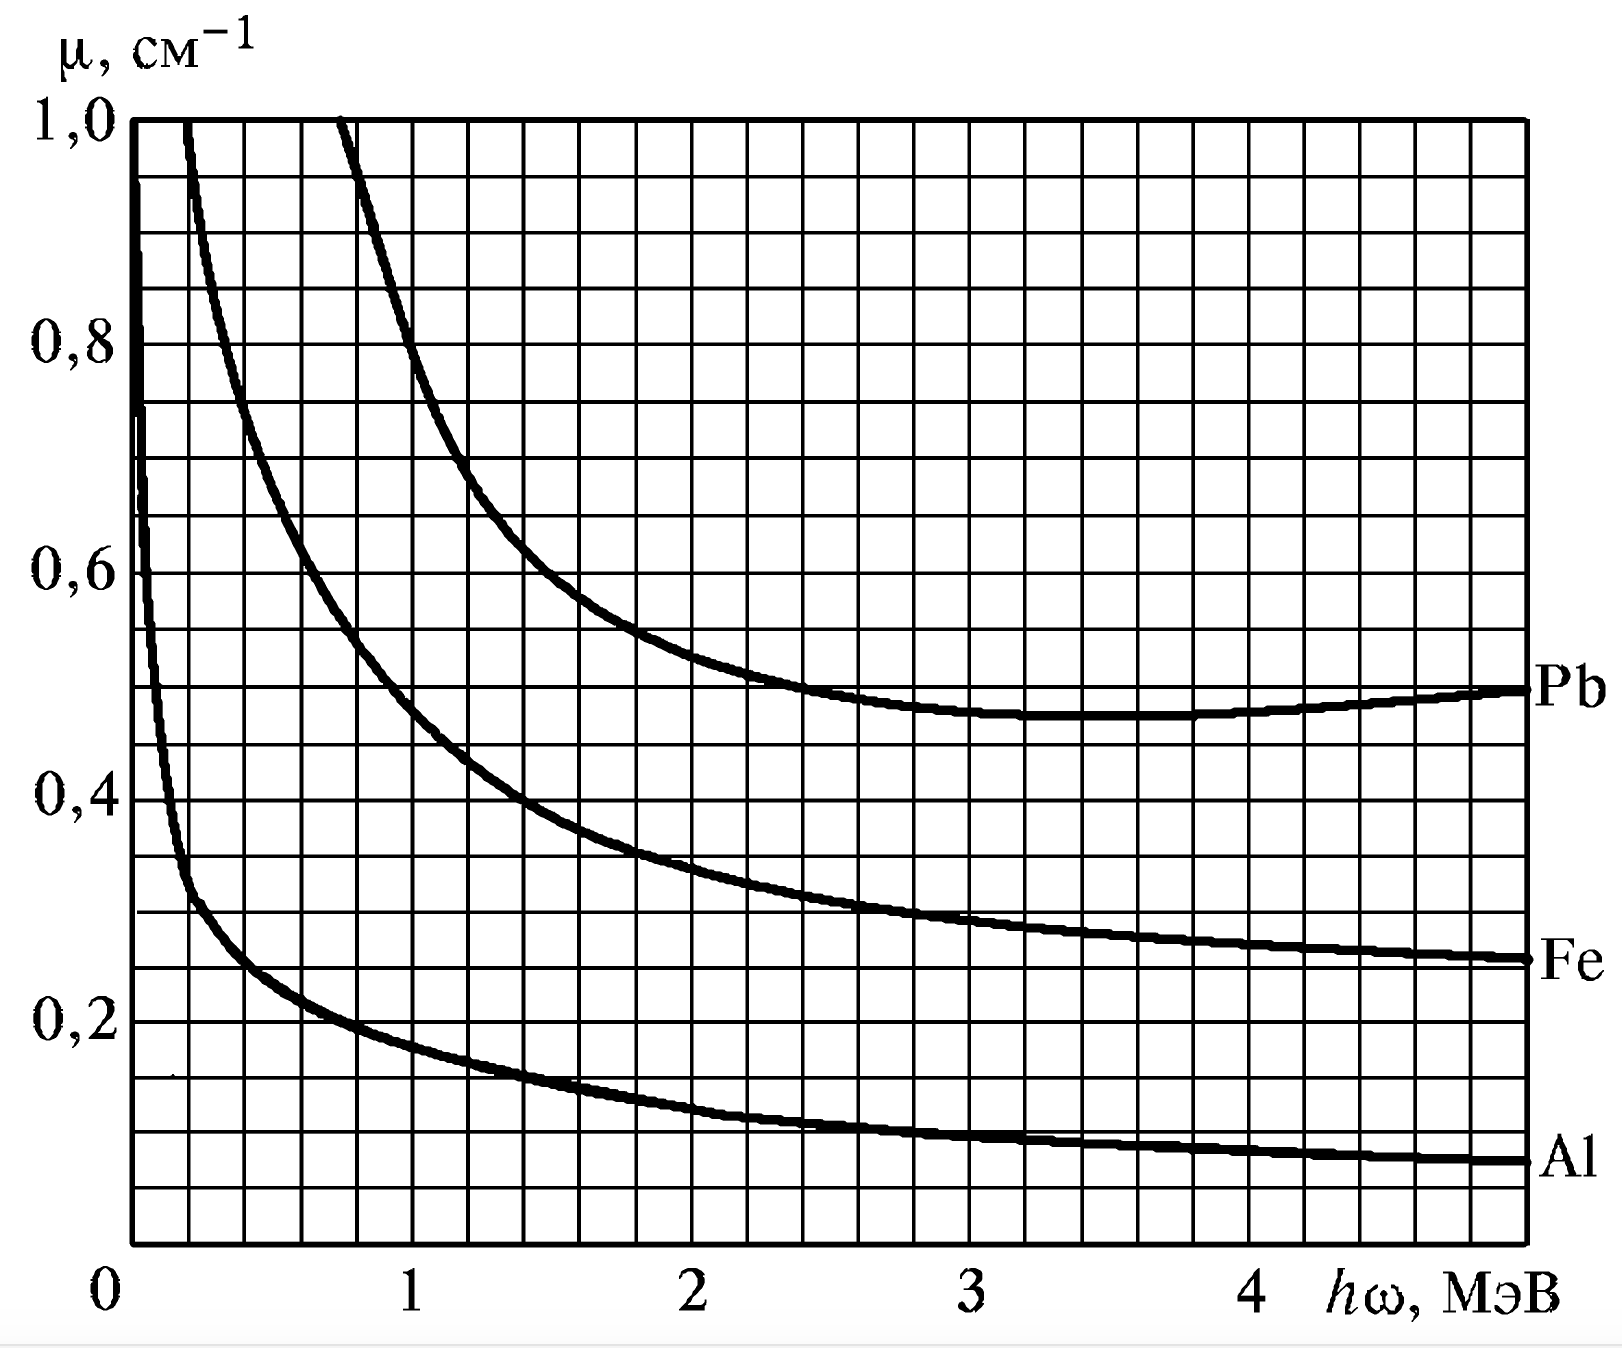
\includegraphics[width=0.6\linewidth]{mu}
		\caption{Полные коэффициенты ослабления потока гамма-лучей в алюминии, железе и свинце}
		\label{ris mu}
	\end{figure}
	
	\medskip
	
\noindent Обратимся вновь к формуле \eqref{I(mu)}. Ее нетрудно получить из теоретических соображений. Рассмотрим опыты, поставленные в хорошей
	геометрии, т. е. в условиях, когда исследуется прохождение сквозь вещество узкого параллельного пучка гамма-лучей. В этом случае не только
	фотоэлектрическое поглощение и генерация пар, но и комптоновское
	рассеяние выводит гамма-кванты из пучка.
	Поэтому при прохождении через вещество меняется только количество, но не энергия гамма-квантов в пучке, так что коэффициент $ \mu $, характеризующий поглощение гамма-квантов в веществе, не зависит от длины
	пути. Обозначим через $ -dN $ число гамма-квантов, выбывших из пучка на
	пути $ dl $. Это число пропорционально имеющемуся их числу $ N $ и прой-
	денному пути $ dl $. Имеем, следовательно,
	
	\begin{equation}\label{N}
	-dN = \mu N dl \Rightarrow N = N_0 e^{-\mu l}
	\end{equation}
	
	\medskip
	
\noindent т.е то же самое, что и формула \eqref{I(mu)}. В плохой геометрии, когда рассеянные под небольшими углами
	гамма-кванты остаются в пучке, их спектр с прохождением вещества меняется, и формула \eqref{I(mu)}, вообще говоря, неприменима. Эта формула, однако, работает и в этом случае лучше, чем можно было бы ожидать. Причина хорошего согласия заключается в том, что гамма-кванты с энергией 1 -- 2 МэВ, потерявшие энергию из-за комптоновского рассеяния,
	быстро выбывают из пучка из-за резкого увеличения сечений $ \sigma_\text{ф} $ и $ \sigma_\text{к} $.
	
	\medskip
	
\noindent В данной работе коэффициент ослабления $ \mu $ измеряется в хорошей
	геометрии. Из формулы \eqref{I(mu)} или \eqref{N} имеем
	
	\begin{equation}\label{mu}
	\mu = \dfrac{1}{l} \ln{\dfrac{N_0}{N}}
	\end{equation}
	
\noindent Для определения коэффициента ослабления нужно, таким образом, измерить толщину образца $ l $, число падающих частиц $ N_0 $ и число
	частиц $ N $, прошедших через образец.
	
	\section{Экспериментальная установка}
	
		\begin{figure}[h!]
		\centering
		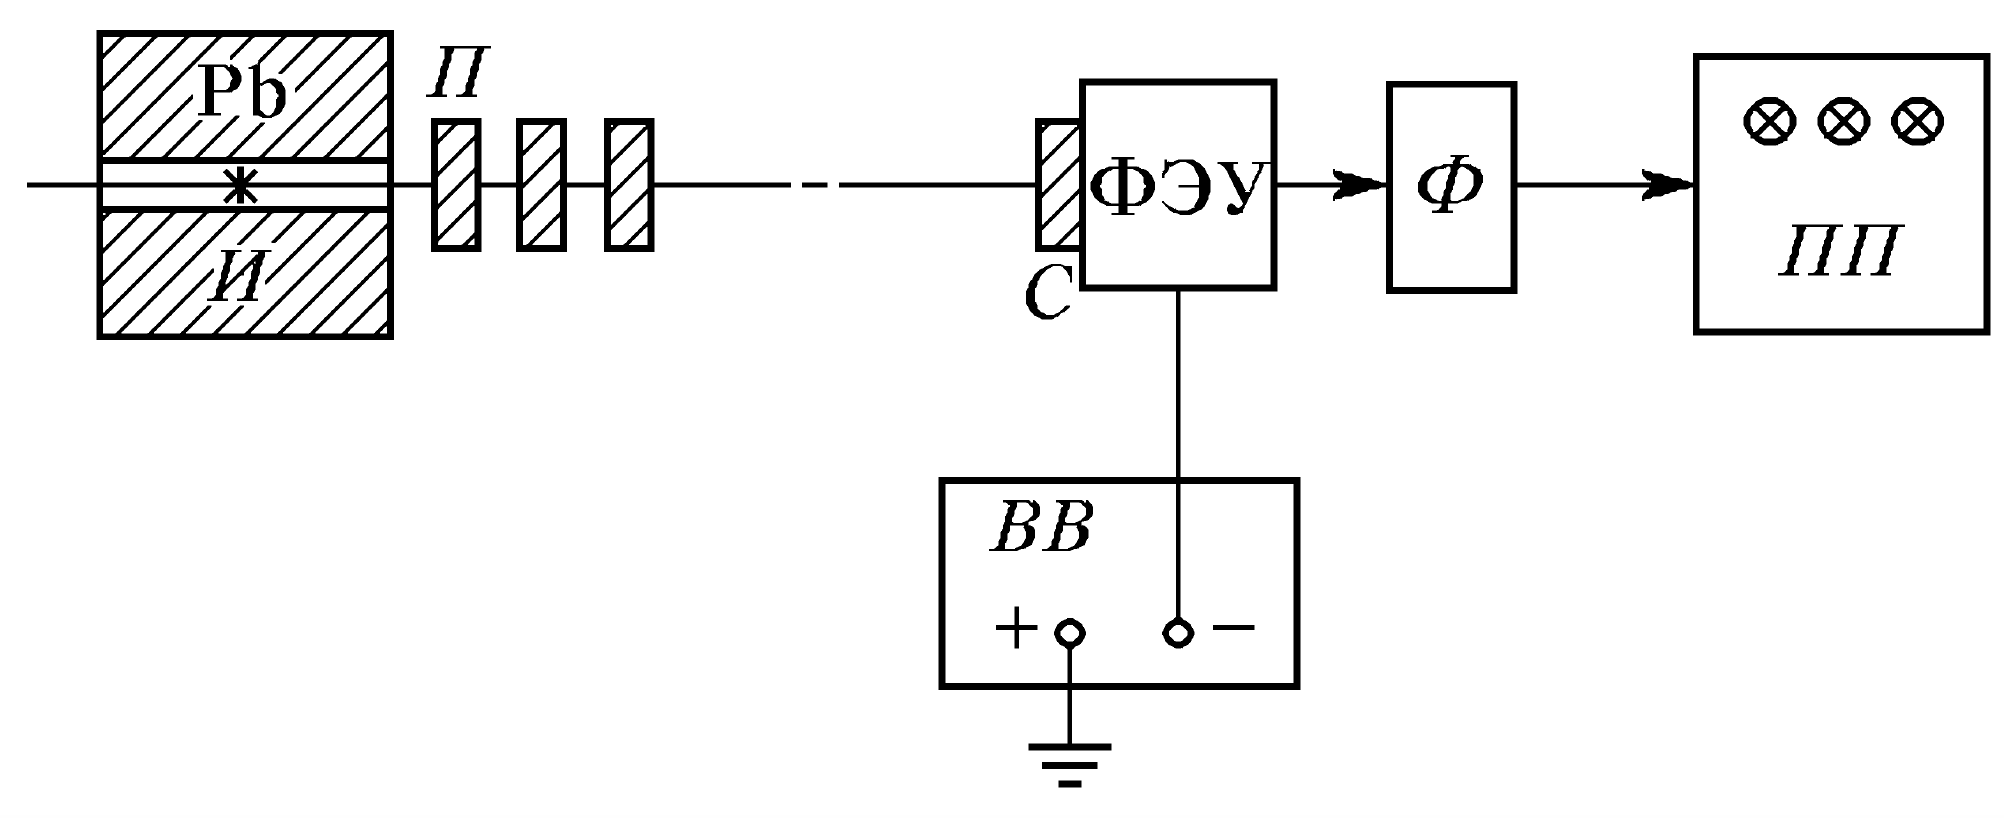
\includegraphics[width=0.7\linewidth]{lab}
		\caption{Блок-схема установки, используемой для измерения коэффициентов ослабления потока гамма-лучей: И --- источник гамма-лучей; $ Pb $ --- свинцовый контейнер с коллиматорным каналом; П --- набор поглотителей; С --- сцинтиллятор (кристалл
			NaI(Tl) ); Ф --- формирователь-выпрямитель}
		\label{ris lab}
	\end{figure}

\noindent Схема установки, используемой в работе, показана на рис. \ref{ris lab}. Свинцовый коллиматор выделяет узкий почти параллельный пучок гамма-квантов, проходящий через набор поглотителей П и регистрируемый сцинтилляционным счетчиком). Сигналы от счетчика усиливаются и регистрируются пересчетным прибором ПП. Высоковольтный выпрямитель ВВ обеспечивает питание сцинтилляционного счетчика.

\medskip

\noindent При недостаточно хорошей геометрии в результаты опытов могут
вкрасться существенные погрешности. В реальных установках всегда имеется конечная вероятность того, что гамма-квант провзаимодействует в
поглотителе несколько раз до того, как попадет в детектор. Чтобы уменьшить число таких случаев, в данной работе сцинтилляционный счетчик расположен на большом расстоянии от источника гамма-квантов, а поглотители имеют небольшие
размеры. Их следует устанавливать за коллиматорной щелью на некотором расстоянии друг от друга, чтобы испытавшие комптоновское
рассеяние и выбывшие из прямого потока кванты с меньшей вероятностью могли в него вернуться.

\newpage

\section{Ход работы}

\noindent 1. Включим пересчетный прибор и высоковольтный выпрямитель, дадим им прогреться.

\medskip

\noindent 2. Убедимся, что установка чувствует $\gamma-$лучи. Для этого измерим скорость счета при полностью открытом коллиматоре, а также при коллиматоре, закрытом свинцовой пробкой. Наблюдаем резкое уменьшение скорости счета.

\medskip

\noindent 3. Исследуем поглощение $\gamma-$лучей в свинце, железе, алюминии и неизвестном образце при различных толщинах образцов. Таблицы с данными см. в Приложении.

\medskip

\noindent Построим кривые зависимости логарифма числа сосчитанных частиц от толщины образца для всех исследуемых веществ.

\medskip

\begin{figure}[h!]
		\centering
		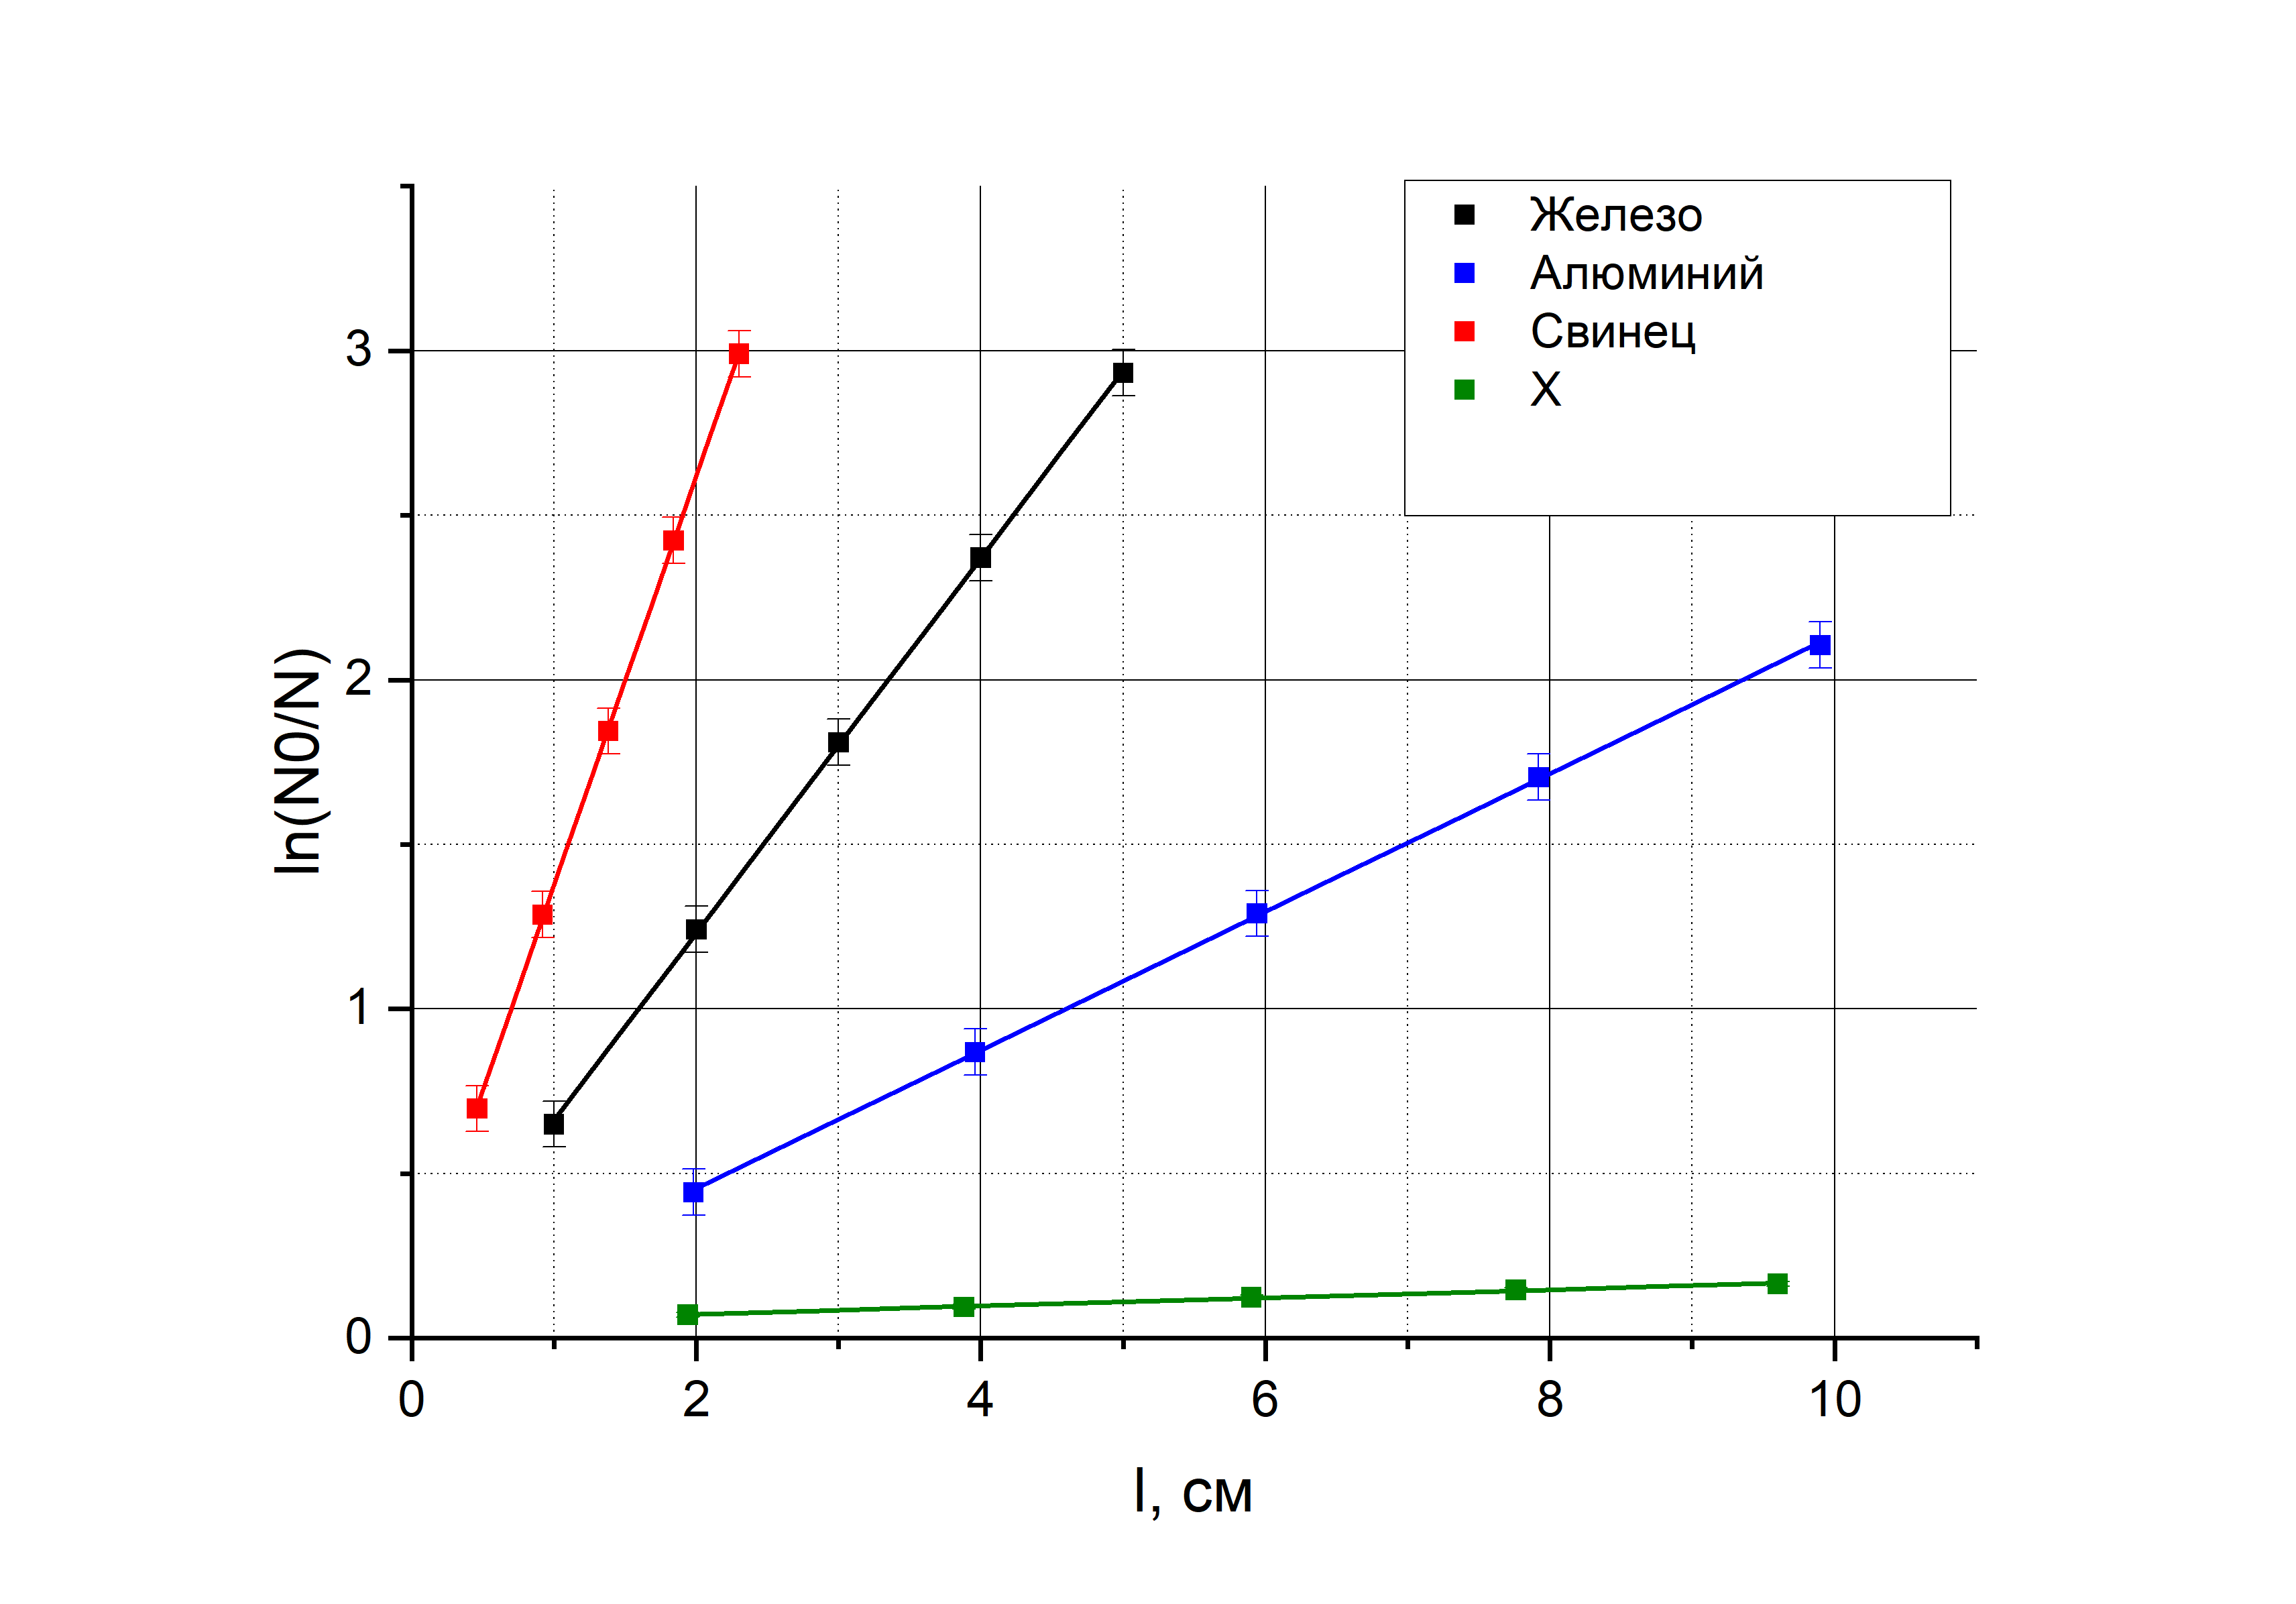
\includegraphics[width=0.99\linewidth]{graph.png}
		\caption{Зависимости логарифма числа сосчитанных частиц от толщины образца для исследуемых веществ}
		
	\end{figure}

\medskip

\noindent Найдем графически коэффициенты ослабления (по коэффициентам наклона прямых), а также рассчитаем $\mu'$.

\medskip

\begin{table}[h!]
\begin{tabular}{|l|l|l|l|l|l|}
\hline
Образец  & $\mu, \text{см}^{-1}$ & $\sigma_{\mu}, \text{см}^{-1}$ & $\rho, \text{г}/\text{см}^3$ & $\mu', \text{см}^{2}/\text{г}$ & $\sigma_{\mu'}, \text{см}^{2}/\text{г}$ \\ \hline
Алюминий & 0,2101                & 0,0014                         & 2,7                          & 0,077815                       & 0,0005                                  \\ \hline
Железо   & 0,5694                & 0,0036                         & 7,874                        & 0,072314                       & 0,0005                                  \\ \hline
Свинец   & 1,2443                & 0,0054                         & 11,34                        & 0,109727                       & 0,0005                                  \\ \hline
X        & 0,0124                & 0,0005                         & -                            & -                              & -                                       \\ \hline
\end{tabular}

\caption{Коэффициенты $\mu$ и $\mu'$}
\end{table}

\medskip

\noindent 4. Используя найденные коэффициенты ослабления по графику (Рис. 2) и табличным данным из Лабораторного практикума (Рис. 5) определим среднюю энергию $\gamma-$лучей, испускаемых источником.

\medskip

\begin{figure}[h!]
		\centering
		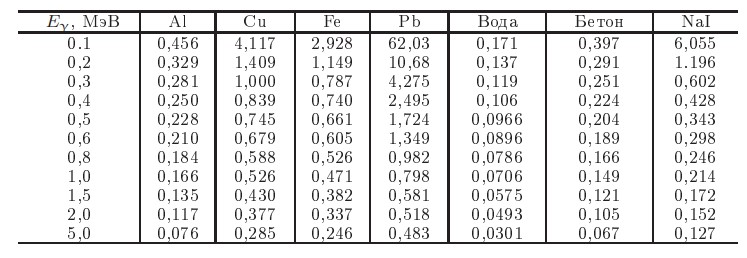
\includegraphics[width=0.90\linewidth]{энергии.jpg}
		\caption{Линейные коэффициенты поглощения $\gamma-$лучей в различных веществах (с см$^{-1}$)}
		
	\end{figure}

\medskip

\noindent Видим, что полученные экспериментально значения лежат в диапазоне энергий от 0,6 до 0,8 МэВ. Средняя энергия $\gamma-$лучей, испускаемых источником составляет $E_{\gamma}$ = 0,7 МэВ.


\medskip

\noindent 5. В работе мы устанавливали поглотитель вплотную к приемнику. Оценим влияние фона в случае, когда поглотитель и приемник находятся на некотором расстоянии: при слое поглотителя толщиной $\approx$ 10 см (алюминий) влияние фона составляет $56\%$. 

\medskip

\noindent Рассмотрим также случай, когда приемник расположен под углом 90 градусов к источнику. Тогда на расстоянии 5,5 см $N = 19438$, при 37 см $N = 5619$. Влияние фона в данном случае составляет $71\%$.

\medskip

\noindent 6. Изучим установку с точки зрения радиационной безопасности. Измерения дозиметром показывают следующие результаты:

\medskip

\begin{table}[h!]
\begin{tabular}{|l|c|c|c|}
\hline
\multirow{2}{*}{}          & Показания         & Показания           & \multirow{2}{*}{T, дни} \\
                           & дозиметра, мкЗв/ч & дозиметра, мкЗв/год &                         \\ \hline
Вход в аудиторию           & 0,16              & 1401,6              & 260                     \\ \hline
Слой алюминия 10 см        & 6,52              & 57115,2             & 7                       \\ \hline
Рассеяние без заслонки     & 1,36              & 11913,6             & 31                      \\ \hline
Рассеяние, 10 см алюминия & 0,58              & 5080,8              & 72                      \\ \hline
\end{tabular}
\end{table}

\medskip

\noindent Учитывая, что годовая норма составляет 1000 мкЗв/год, рассчитаем сколько времени нужно находиться в данных местах и условиях, чтобы ее получить. Результаты также занесем в таблицу.

\section{Вывод}

В ходе работы было изучено ослабление потоков гамма-квантов в четырех различных веществах: алюминии, железе, свинце и неизвестном веществе, внешне похожем на пробку. Экспериментально с помощью сцинтилляционного счетчика получены коэффициенты ослабления этих веществ. Также с помощью табличных данных была определена средняя энергия гамма-квантов - 0,7 МэВ.

\newpage

\section{Приложение}

\begin{table}[h!]

\begin{center}

\begin{tabular}{|llllll|}
\hline
\multicolumn{6}{|c|}{Алюминий}                                                                                                                                               \\ \hline
\multicolumn{1}{|l|}{N}      & \multicolumn{1}{l|}{t, с} & \multicolumn{1}{l|}{l, см} & \multicolumn{1}{l|}{$\sigma_l,$ см} & \multicolumn{1}{l|}{$ln(N_0/N)$} & $\sigma_{ln(N_0/N)}$ \\ \hline
\multicolumn{1}{|l|}{242478} & \multicolumn{1}{l|}{60}   & \multicolumn{1}{l|}{1,98}  & \multicolumn{1}{l|}{0,20}           & \multicolumn{1}{l|}{0,443449}    & 0,007       \\ \hline
\multicolumn{1}{|l|}{159065} & \multicolumn{1}{l|}{60}   & \multicolumn{1}{l|}{3,96}  & \multicolumn{1}{l|}{0,30}           & \multicolumn{1}{l|}{0,869348}    & 0,008       \\ \hline
\multicolumn{1}{|l|}{105084} & \multicolumn{1}{l|}{60}   & \multicolumn{1}{l|}{5,94}  & \multicolumn{1}{l|}{0,35}           & \multicolumn{1}{l|}{1,290357}    & 0,007       \\ \hline
\multicolumn{1}{|l|}{70146}  & \multicolumn{1}{l|}{60}   & \multicolumn{1}{l|}{7,92}  & \multicolumn{1}{l|}{0,40}           & \multicolumn{1}{l|}{1,704089}    & 0,007       \\ \hline
\multicolumn{1}{|l|}{47584}  & \multicolumn{1}{l|}{60}   & \multicolumn{1}{l|}{9,9}   & \multicolumn{1}{l|}{0,50}           & \multicolumn{1}{l|}{2,105953}    & 0,007       \\ \hline
\end{tabular}

\end{center} 

\caption{Поглощение при различных толщинах образца для алюминия}
\end{table}


\begin{table}[h!]
\begin{center}
\begin{tabular}{|llllll|}
\hline
\multicolumn{6}{|c|}{Железо}                                                                                                                                                          \\ \hline
\multicolumn{1}{|l|}{N}      & \multicolumn{1}{l|}{t, с} & \multicolumn{1}{l|}{l, см} & \multicolumn{1}{l|}{$\sigma_l,$ см} & \multicolumn{1}{l|}{$ln(N_0/N)$} & $\sigma_{ln(N_0/N)}$ \\ \hline
\multicolumn{1}{|l|}{197558} & \multicolumn{1}{l|}{60}   & \multicolumn{1}{l|}{1}     & \multicolumn{1}{l|}{0,20}           & \multicolumn{1}{l|}{0,65019}     & 0,007                \\ \hline
\multicolumn{1}{|l|}{110198} & \multicolumn{1}{l|}{60}   & \multicolumn{1}{l|}{2}     & \multicolumn{1}{l|}{0,30}           & \multicolumn{1}{l|}{1,241953}    & 0,007                \\ \hline
\multicolumn{1}{|l|}{63292}  & \multicolumn{1}{l|}{60}   & \multicolumn{1}{l|}{3}     & \multicolumn{1}{l|}{0,35}           & \multicolumn{1}{l|}{1,81004}     & 0,006                \\ \hline
\multicolumn{1}{|l|}{36961}  & \multicolumn{1}{l|}{60}   & \multicolumn{1}{l|}{4}     & \multicolumn{1}{l|}{0,40}           & \multicolumn{1}{l|}{2,371063}    & 0,006                \\ \hline
\multicolumn{1}{|l|}{21926}  & \multicolumn{1}{l|}{60}   & \multicolumn{1}{l|}{5}     & \multicolumn{1}{l|}{0,50}           & \multicolumn{1}{l|}{2,932581}    & 0,007                \\ \hline
\end{tabular}

\end{center}

\caption{Поглощение при различных толщинах образца для железа}
\end{table}


\begin{table}[h!]
\begin{center}

\begin{tabular}{|llllll|}
\hline
\multicolumn{6}{|c|}{Свинец}                                                                                                                                                          \\ \hline
\multicolumn{1}{|l|}{N}      & \multicolumn{1}{l|}{t, с} & \multicolumn{1}{l|}{l, см} & \multicolumn{1}{l|}{$\sigma_l,$ см} & \multicolumn{1}{l|}{$ln(N_0/N)$} & $\sigma_{ln(N_0/N)}$ \\ \hline
\multicolumn{1}{|l|}{188557} & \multicolumn{1}{l|}{60}   & \multicolumn{1}{l|}{0,46}  & \multicolumn{1}{l|}{0,22}           & \multicolumn{1}{l|}{0,697303}    & 0,007                \\ \hline
\multicolumn{1}{|l|}{105464} & \multicolumn{1}{l|}{60}   & \multicolumn{1}{l|}{0,92}  & \multicolumn{1}{l|}{0,36}           & \multicolumn{1}{l|}{1,286678}    & 0,007                \\ \hline
\multicolumn{1}{|l|}{61225}  & \multicolumn{1}{l|}{60}   & \multicolumn{1}{l|}{1,38}  & \multicolumn{1}{l|}{0,38}           & \multicolumn{1}{l|}{1,844327}    & 0,007                \\ \hline
\multicolumn{1}{|l|}{35165}  & \multicolumn{1}{l|}{60}   & \multicolumn{1}{l|}{1,84}  & \multicolumn{1}{l|}{0,41}           & \multicolumn{1}{l|}{2,423752}    & 0,007                \\ \hline
\multicolumn{1}{|l|}{20801}  & \multicolumn{1}{l|}{60}   & \multicolumn{1}{l|}{2,3}   & \multicolumn{1}{l|}{0,50}           & \multicolumn{1}{l|}{2,9906}      & 0,007                \\ \hline
\end{tabular}

\end{center}

\caption{Поглощение при различных толщинах образца для свинца}
\end{table}



\begin{table}[h!]
\begin{center}

\begin{tabular}{|llllll|}
\hline
\multicolumn{6}{|c|}{Неизвестный образец}                                                                                                                                                          \\ \hline
\multicolumn{1}{|l|}{N}      & \multicolumn{1}{l|}{t, с} & \multicolumn{1}{l|}{l, см} & \multicolumn{1}{l|}{$\sigma_l,$ см} & \multicolumn{1}{l|}{$ln(N_0/N)$} & $\sigma_{ln(N_0/N)}$ \\ \hline
\multicolumn{1}{|l|}{350907} & \multicolumn{1}{l|}{60}   & \multicolumn{1}{l|}{1,94}  & \multicolumn{1}{l|}{0,20}           & \multicolumn{1}{l|}{0,071314}    & 0,007                \\ \hline
\multicolumn{1}{|l|}{342912} & \multicolumn{1}{l|}{60}   & \multicolumn{1}{l|}{3,88}  & \multicolumn{1}{l|}{0,33}           & \multicolumn{1}{l|}{0,094493}    & 0,007                \\ \hline
\multicolumn{1}{|l|}{332916} & \multicolumn{1}{l|}{60}   & \multicolumn{1}{l|}{5,9}   & \multicolumn{1}{l|}{0,47}           & \multicolumn{1}{l|}{0,12425}     & 0,007                \\ \hline
\multicolumn{1}{|l|}{325554} & \multicolumn{1}{l|}{60}   & \multicolumn{1}{l|}{7,76}  & \multicolumn{1}{l|}{0,48}           & \multicolumn{1}{l|}{0,146746}    & 0,007                \\ \hline
\multicolumn{1}{|l|}{319857} & \multicolumn{1}{l|}{60}   & \multicolumn{1}{l|}{9,6}   & \multicolumn{1}{l|}{0,53}           & \multicolumn{1}{l|}{0,164509}    & 0,007                \\ \hline
\end{tabular}


\end{center}

\caption{Поглощение при различных толщинах для неизвестного образца}
\end{table}

\end{document}